\documentclass[10pt, a4paper]{scrartcl}

\usepackage{vorschule}
\usepackage[
    typ=ab,
    fach=Mathematik,
    lerngruppe={Q2-GK},
    nummer=4,
    module={Symbole,Lizenzen},
    seitenzahlen=keine,
    farbig,
    lizenz=cc-by-nc-sa-4,
]{schule}

\usepackage[
	kuerzel=Ngb,
	reihe={Analytische Geometrie},
	version={2019-09-22},
]{ngbschule}

\author{J. Neugebauer}
\title{Bewegung eines U-Boots}
\date{\Heute}

\setzeAufgabentemplate{ngbnormal}

%\usepackage{qrcode}
%\usepackage{tinspire}


\begin{document}

\ReiheTitel
\begin{aufgabe}
	\begin{wrapfigure}{r}{4cm}
		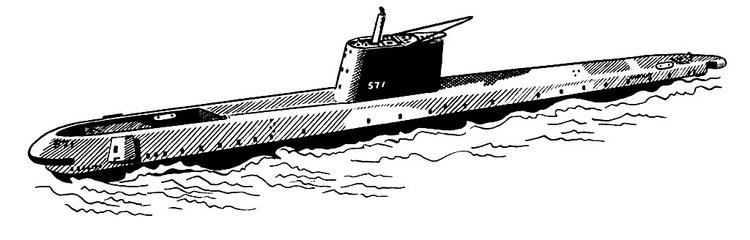
\includegraphics[width=4cm]{Q2-AB.4-Abb_U-Boot.jpg}
	\end{wrapfigure}
	Ein militärisches U-Boot wurde von einer Beobachtungsstation im Punkt $U\pkt*(1000|2000|-300)$ 
	gesichtet (Angaben in \si{\meter} relativ zur Station). Laut Beobachtung bewegt es sich pro Minute
	um den Vektor $\vec{v} = \begin{pmatrix} 320 \\ -250 \\ 55 \end{pmatrix}$ fort.
		
	\begin{teilaufgaben}
		\teilaufgabe Bestimmen sie die wahrscheinliche Position des U-Boots nach einer, zwei, dreieinhalb und fünf Minuten. Bestimmen sie die Position relativ zum Ausgangspunkt $U$,
		sowie zur Beobachtungsstation (dem Koordinatenursprung).
		\teilaufgabe Skizzieren sie die Punkte in einem Koordinatensystem mit geeignetem Maßstab. 
		Verdeutlichen sie die Bewegung des U-Bootes.
		\teilaufgabe Stellen sie eine allgemeine Formel zur Berechnung des Ortsvektors $OX$ der Position $X$ des U-Boots nach $t$ Minuten auf (relativ zu $U$ und zum Ursprung). Beschreiben sie ihr vorgehen.
		\teilaufgabe\symStern Wann erreicht das U-Boot die Oberfläche und welche Position hat es zu diesem Zeitpunkt? Welche Strecke hat es dann von seinem Startpunkt zurück gelegt?
	\end{teilaufgaben}
\end{aufgabe}



\end{document}
